%%%%%%%%%%%%%%%%%%%%%%%%%%%%%%%%%%%%%%%%%%%%%%%%%%%%%%%%%%%%%%%%%%%%%%%%%%%%
%% Trim Size : 11in x 8.5in
%% Text Area : 9.6in (include Runningheads) x 7in
%% ws-jai.tex, 26 April 2012
%% Tex file to use with ws-jai.cls written in Latex2E.
%% The content, structure, format and layout of this style file is the
%% property of World Scientific Publishing Co. Pte. Ltd.
%%%%%%%%%%%%%%%%%%%%%%%%%%%%%%%%%%%%%%%%%%%%%%%%%%%%%%%%%%%%%%%%%%%%%%%%%%%%
%%

%\documentclass[draft]{ws-jai}
\documentclass{ws-jai}
\usepackage[flushleft]{threeparttable}
\def\btex{B{\sc IB}\TeX\ }
\begin{document}

\catchline{}{}{}{}{} % Publisher's Area please ignore

\markboth{Jack Hickish, CASPER gang, etc.}{The Collaboration for Astronomy Signal Processing and Electronics Research in 2016.}

\title{The Collaboration for Astronomy Signal Processing and Electronics Research in 2016}

%\author{First Author$^\dagger$, Second Author$^\ddagger$, Third Author$^\ddagger$ and Fourth Author$^\S$}
\author{Jack Hickish$^\dagger$, Others$^\ddagger$}

\address{
$^\dagger$Radio Astronomy Laboratory, UC Berkeley, Berkeley, CA 94720, USA, jackh@astro.berkeley.edu\\
$^\ddagger$Group, Company, Address, City, State ZIP/Zone, Country\\
$^\S$Group, Company, Address, City, State ZIP/Zone, Country, fauthor@company.com
}

\maketitle

\corres{$^\dagger$Jack Hickish}

\begin{history}
\received{(to be inserted by publisher)};
\revised{(to be inserted by publisher)};
\accepted{(to be inserted by publisher)};
\end{history}

\begin{abstract}

The Collaboration for Astronomy Signal Processing and Electronics Research
(CASPER) has been working for a decade to reduce the time and cost of designing,
building and deploying new digital radio astronomy instruments.  Today,
CASPER-designed hardware powers some ?? scientific instruments worldwide, and
are used by scientists and engineers at ?? academic institutions.  In this paper
we summarize the current offerings of the CASPER collaboration, focussing on
currently-available and next-generation hardware.  We describe the ongoing state
of software development, as CASPER looks to support an ever-increasing selection
of off-the-shelf digital signal processing platforms.

\end{abstract}

\keywords{CASPER, digital signal processing, radio astronomy, instrumentation}

\section{Introduction}

Since the first digital instrument used in radio astronomy \citep{Weinreb} we
have seen a growing adoption of digital processing hardware as the foundation on
which radio telescopes are built.  Today, CPUs, GPUs, FPGAs and ASICs power
almost all of the world's radio telescopes, and our ability to do science has
become inextricably linked with our ability to perform digital computation.
With the capability of digital processing hardware scaling exponentially with
Moore's law, the ability to leverage current technology by reducing the
design-time of new instruments is critical in effective deployments of new radio
astronomy instruments.

The Collaboration for Astronomy Signal Processing and Electronics Research
(CASPER) puts \emph{time-to-science}, the time between conception of an
instrument and its deployment, as a central figure of merit in instrument
design. CASPER works to minimize time-to-science by working to develop and
support open-source, general-purpose hardware, software libraries and
programming tools which allow rapid instrument design, and straightforward
upgrade cycles.

With CASPER hardware and software now powering some ?? radio astronomy
instruments worldwide (see Table~\ref{table:casper-instruments}) including some
of the largest, most advanced telescopes ever built, such as the upcoming
MeerKat Array \citep{MeerKAT}, it is appropriate to document the state of the
Collaboration.

In this paper, we first summarize the design philosophy of CASPER in
Section~\ref{sec:CASPER-philosophy}.  In Section~\ref{sec:Hardware} we describe
currently available CASPER hardware offerings, including the range of digitizers
developed and supported by CASPER. Key to CASPER's success are the firmware
libraries and programming infrastructure provided by the collaboration, which we
overview in Section~\ref{sec:Software}.  In Section~\ref{sec:Deployments} we
document the extensive and wide-ranging applications to which CASPER hardware
and design-tools have been applied. Finally, we describe the future direction of
and challenges faced by the CASPER collaboration in Section~\ref{sec:Future},
with concluding remarks in Section~\ref{sec:Conclusions}.

\section{The CASPER Philosophy} \label{sec:CASPER-philosophy}

World-wide, radio astronomy is a relatively small industry and has minimal financial incentive attracting investors. This means that often institutions often rely heavily on government funding. It is therefore beneficial to share resources between organisations as to leverage the work that others have put into developing radio astronomy instrumentation. For this reason institutions often open source their intellectual property. CASPER was founded to aid this collaboration. It aims to share and collaborate on both hardware and software for the design of radio astronomy DSP systems.

The CASPER community has designed multiple FPGA based hardware platforms and the software tools to design and support these platforms.

Along with hardware platforms, CASPER provides a tool-flow based on the Matlab, Simulink and XSG tools to enable a designer to easily design and target a particular hardware platform. \cite{p_mcmahon} The interface is a graphical design environment in Simulink where a designer can drag and drop blocks and connect them with wires in the desired configuration. A library of CASPER DSP blocks are provided. These are targeted at the particular type of DSP typical of radio astronomy data processing. In addition, there is also a library of hardware specific blocks, which contain the controllers for ADCs and Ten Gigabit Ethernet (TGE) modules, amongst others. The flow provides a "One-Click" solution from design to bitstream, ready to upload onto a board. The DSP parts of the design are easily transferable to other Xilinx FPGA hardware. This eases upgrades to new hardware, as well as aiding collaboration between teams using different CASPER hardware platforms. \cite{casper_paper} 

CASPER makes use of Ethernet as a generic backplane architecture, to provide packetised interconnects between hardware modules. In this way, instruments can consist of different types of data processing hardware. For example, it is easy to hand off parts of the processing chain to a GPU cluster by redirecting the data sent over the network to different Internet Protocol (IP) address. A design can even leverage the IP Multicast protocol\footnote{IP multicast is described in RFC 1112} which allows additional instruments to subscribe to the data and process it concurrently alongside the main instrument. This keeps the problem of full cross-bar interconnects in the domain of the switch manufactures and allows instrument designers to focus on digital signal processing. \cite{manley2014} \cite{parsons2005}

Overall, CASPER has a progressive philosophy towards instrumentation design and it is important to take into account when examining, designing and implementing tools to be used by this community and others.

\subsection{Computing by the yard}

\subsection{Ethernet}

\subsubsection{Multicast \& Commensal Instruments}


\section{CASPER Hardware} \label{sec:Hardware}

Since its inception, the collaboration has produced a range of hardware with particular focus on FPGA boards and supporting hardware such as Analog-to-digital Converters (ADC) and Ethernet mezzanine cards. 

\subsection{FPGA platforms}

Much of the focus of the community has moved from the popular ROACH2 platform to the newer SNAP and SKARAB boards which sport the Xilinx Kintex and Virtex FGPAs respectively.

\subsubsection{ROACH1}

For completeness it is important to mention the grandfather of the current hardware generation, the ROACH1. The architecture is based on a single FPGA with a control processor and mezzanine connectors for the addition of ADCs and other peripherals. \cite{} The core of the ROACH is the Xilinx Virtex 5 xc5vlx110t chip. The CASPER tools still provide support for this board even though it is 2 generations old.

%% Wesley New

\subsubsection{ROACH2}

The ROACH2 is the update to the ROACH platform, the major differences being the Virtex 6 FPGA and the addition of two mezzanine slots which could be used for memory or ethernet cards.
%% Wesley New

\subsubsection{SKARAB}

The Square Kilometre Array Reconfigurable Application Board (SKARAB) hardware is the next generation FPGA hardware platform that has been designed by a South African company, Peralex, according to the specifications of SKA-SA, as an alternative to the ROACH2 hardware for applications requiring better processing performance. The departure from the ``ROACH'' naming convention to the ``SKARAB'' naming convention is because the interfaces between the ROACH2 and the SKARAB are not compatible.

A functional block diagram of the SKARAB is presented in Figure~\ref{fig:skarab_bd} \cite{cliff16}.

\begin{figure}[h]
\centering
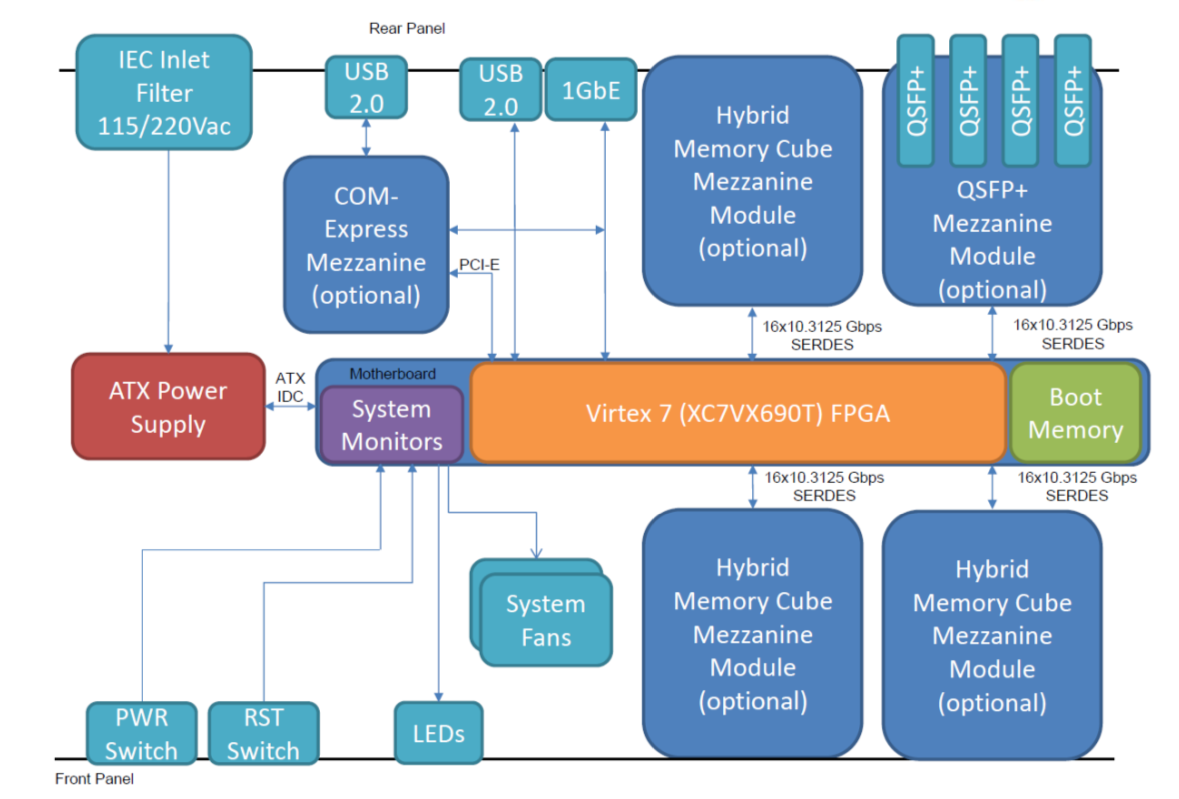
\includegraphics[width=150mm, scale=0.5]{skarab_bd}
\caption{SKARAB Functional Block Diagram}
\label{fig:skarab_bd}
\end{figure}

At the heart of the SKARAB processing, lies the Xilinx Virtex 7 FPGA (XC7VX690T). This FPGA consists of 693120 logic cells, 52 Mb of internal random access memory (RAM) blocks and 3600 digital signal processing (DSP) slices \cite{cliff16}. Nearly all of the input/output (I/O) available is high-speed serial/deserializer (SERDES) I/O \cite{Teag15}. 

The SKARAB makes provision for four mezzanine sites with each site interfacing with sixteen transmit and sixteen receive 10 Gbps SERDES lines \cite{cliff16}. This means each site can handle a throughput of 160 Gbps and if all the sites are utilized, a total of 640 Gbps can be achieved.

There is no power personal computer (PPC), but provision has been made for the COM Express mezzanine site which can interface with an external processor via single lane PCIe \cite{Teag15}.
 
The SKARAB has already been tested with two existing mezzanine cards: QSFP+ Mezzanine Module and the Hybrid Memory Cube (HMC) Mezzanine Module. The Peralex QSFP+ Mezzanine Module supports four 40Gb Ethernet interfaces and the SKA-SA HMC Mezzanine module provides external memory storage for the processing using high speed serial memory \cite{cliff16}.     

The hardware of the SKARAB is presented in Figure~\ref{fig:skarab_hw} \cite{cliff16}.

\begin{figure}[h]
\centering
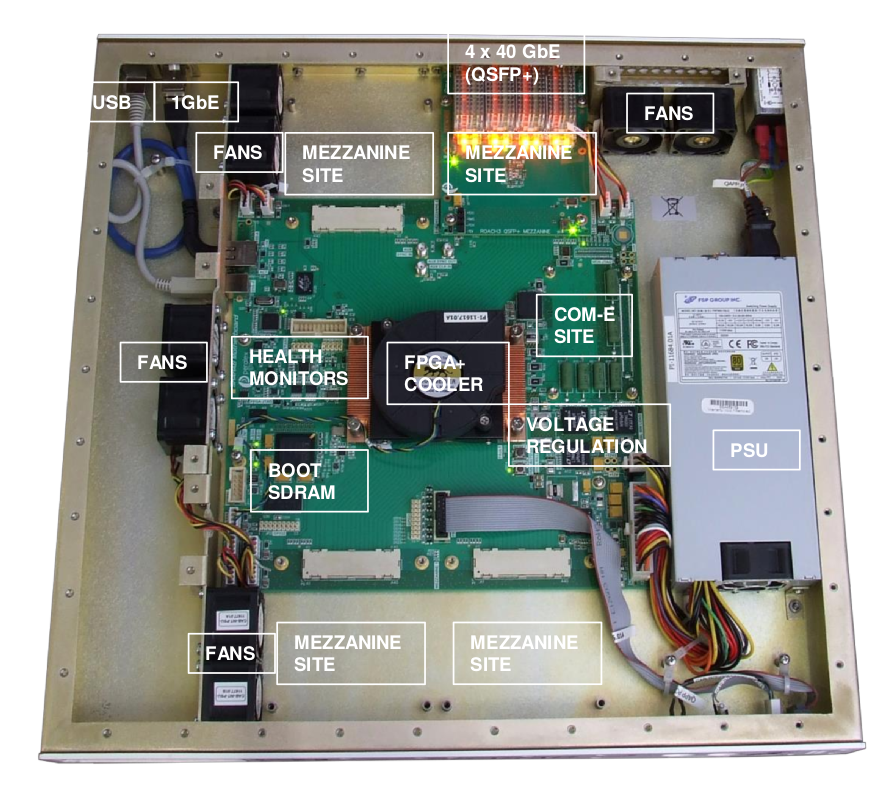
\includegraphics[width=150mm, scale=0.5]{skarab_hw}
\caption{SKARAB Hardware}
\label{fig:skarab_hw}
\end{figure}

The SKARAB board support package (BSP) comes with the 40GbE core, 1GbE core, HMC core and the management microcontroller, which runs on the FPGA (Xilinx's microblaze processor) \cite{cliff16}. The management microcontroller sets up the network (1GbE, 40GbE), performs FPGA configuration (1GbE), monitors the voltages and currents, monitors and controls the fan speeds and handles communication to/from the FPGA via the wishbone bus \cite{cliff16} \cite{Teagu15}.
 
The SKARAB BSP is currently being added to the CASPER tool flow and should be ready in December 2016.
SKA-SA will be integrating 300 SKARAB units, as part of the MeerKAT upgrades, and should be ready for operation latest by the end of 2017.

%% Adam Isaacson

\subsubsection{SNAP}

\subsection{ADCs \& DACs}


\section{CASPER Software \& Programming Tools} \label{sec:Software}

\subsection{The CASPER Tool Flow}

%% Wesley New

\subsection{JASPER Tool Flow}

%% Jack Hickish to introduce this and explain history

%% Adam Isaacson to explain the latest additions
The JASPER tool flow is currently being upgraded to make provision for additional front ends and back ends besides Simulink and Xilinx, respectively. This will prevent the developer from being tied down to a specific software package and FPGA platform \cite{Isaac16}. The current upgrades are presented in Figure~\ref{fig:jasper_ug_bd} \cite{Isaac16}.

\begin{figure}[h]
\centering
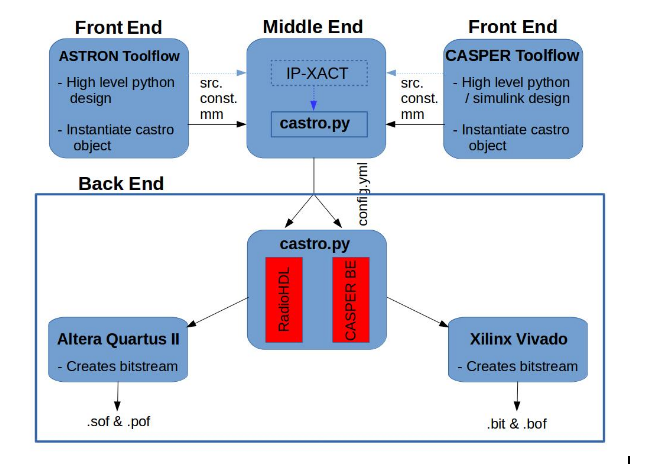
\includegraphics[width=150mm, scale=0.5]{jasper_ug_bd}
\caption{JASPER Upgrade Tool Flow Diagram}
\label{fig:jasper_ug_bd}
\end{figure}  

The Front-End includes the structural VHDL or any modelling tools e.g. Matlab/Simulink, Labview, Sci-Lab/Sci-Cos and MyHDL. It includes a script which will instantiate the python classes inside the Middle End process \cite{Isaac16}. 

The python classes are located in the Middle End (castro.py) file. In the future, it is likely that the Front End will come in through another interface e.g. possibly IP-XACT in order to make provision to interface to other simulation tools e.g. Sci-Cos and Sci-Lab. This interface is denoted by the dashed lines in Figure~\ref{fig:jasper_ug_bd}. IP-XACT is an IEEE standard and is used to integrate different IP packages together, provided that the IP interfacing meets the IP-XACT standard. The IP-XACT interface would be in the form of an XML script. The decision to utilise IP-XACT has not been finalised yet. The castro.py is passed all the Front End memory map, constraints and source files. The castro.py script takes this metadata from the Front End and dumps all of this metadata into a YAML configuration file (config.yml). It should be noted that the Middle End module is not platform agnostic due to the hardware and platform metadata \cite{Isaac16}.

The Back End consists of the same castro python class that exists in the Middle End. The castro.py python script will load the config.yml file/metadata and instantiate python objects with this metadata, which will either be sent to RadioHDL if targeting the Altera hardware or the Casper Back End, if targeting the Xilinx hardware. This will also allow the user to target other vendor hardware in the future e.g. Lattice and Actel and due to the common castro.py python script, it will easier to just add an additional back end \cite{Isaac16}. 

The RadioHDL process will then generate the necessary Quartus project files and run the compiler. The output of the process will be the Altera FPGA SRAM Object file (sof) and Programming Object File (pof). The Casper Back End generates the necessary tcl scripts, which runs the Vivado compiler. The output of the process is the Xilinx FPGA bit and Borph Object File (bof) programmable files \cite{Isaac16}.

The current release of the JASPER tool flow actually includes the castro python class and the CASPER back end makes provision for both Xilinx ISE and Vivado. The JASPER tool flow also makes provision for the SKARAB platform and the generation of the fpg configuration files, which are used for the ROACH2 and SKARAB configuration \cite{Balla16}.


%% Adam Isaacson / Jack Hickish

\subsection{CASPER DSP Libraries}

%% Andrew Martens + anyone else keen to contribute

\emph{Just Another Signal Processing EnviRonment}


\section{CASPER Deployments} \label{sec:Deployments}

\subsection{MeerKAT}

%% Ask Ruby van Rooyen

\section{Future Directions \& Challenges} \label{sec:Future}

\subsection{Hardware Design Challenges}

\subsubsection{Timing Closure}

\subsubsection{High Speed Memories} \label{sec: HSM}

%% HMC 

\subsection{Support of off-the-shelf hardware}

\subsection{CPU/GPU programming/data-transport}

\subsection{Design re-use}

\subsection{Observatory Integration}


\section{Conclusions} \label{sec:Conclusions}


\bibliographystyle{ws-jai}

\bibliography{casper-2016}



\end{document} 
